\documentclass[border=3pt]{standalone}
% Preâmbulo compartilhado pelos diagramas TikZ da aula 8 de IHR (Métodos de Pesquisa)
\usepackage[T1]{fontenc}
\usepackage[utf8]{inputenc}
\usepackage{lmodern}
\usepackage{amsmath}
\usepackage{xcolor}
\usepackage{tikz}
\usetikzlibrary{arrows.meta,angles,quotes,decorations.pathmorphing,decorations.pathreplacing,calc,
                positioning,shapes.geometric,shapes.misc,backgrounds,fit,
                math}

% Paleta (mesma dos SVGs originais)
% Paleta da disciplina de IHR: acento azul (#1A6FB5), cor de destaque do tema.
% (o nome "dblue" é mantido para não alterar todos os diagramas)
\definecolor{dblue}{HTML}{1A6FB5}
\definecolor{dorange}{HTML}{B3541E}
\definecolor{dgreen}{HTML}{4A7C59}
\definecolor{dred}{HTML}{9C4B4B}
\definecolor{dcream}{HTML}{F4F1EA}
\definecolor{dshade}{HTML}{DDD7C9}

% Função gaussiana (não normalizada por padrão de escala visual)
\pgfmathdeclarefunction{gauss}{3}{%
  \pgfmathparse{1/(#3*sqrt(2*pi))*exp(-((#1-#2)^2)/(2*#3^2))}%
}

% Estilos comuns (prefixo d... para não colidir com chaves internas do pgf)
\tikzset{
  >={Stealth[length=2mm]},
  dguide/.style={gray!55, dashed, line width=0.4pt},
  daxis/.style={gray!60, line width=0.7pt, ->},
  dbody/.style={fill=black!3, draw=black!80, line width=1pt},
  dacc/.style={draw=dblue, line width=1pt},
  dlbl/.style={black!55, font=\small},
  dsub/.style={black!45, font=\footnotesize},
  dstate/.style={circle, draw=black!80, fill=dcream, line width=1pt,
                 minimum size=17mm, font=\large, inner sep=1pt},
  dobs/.style={circle, draw=black!80, fill=dshade, line width=1pt,
               minimum size=14mm, font=\large, inner sep=1pt},
  dbox/.style={rounded corners=2pt, draw=black!80, fill=dcream, line width=1pt,
               align=center, inner sep=6pt},
  dop/.style={circle, draw=black!80, fill=white, line width=1pt,
              minimum size=6mm, inner sep=0pt, font=\small},
  dtrans/.style={->, dblue, line width=1pt},
  dmeas/.style={->, dorange, line width=1pt},
  dcurve/.style={line width=1pt, dblue},
  dcurveb/.style={line width=1.4pt, dorange},
}

\begin{document}
\hyphenpenalty=10000 \exhyphenpenalty=10000 \tolerance=9999 \emergencystretch=3em
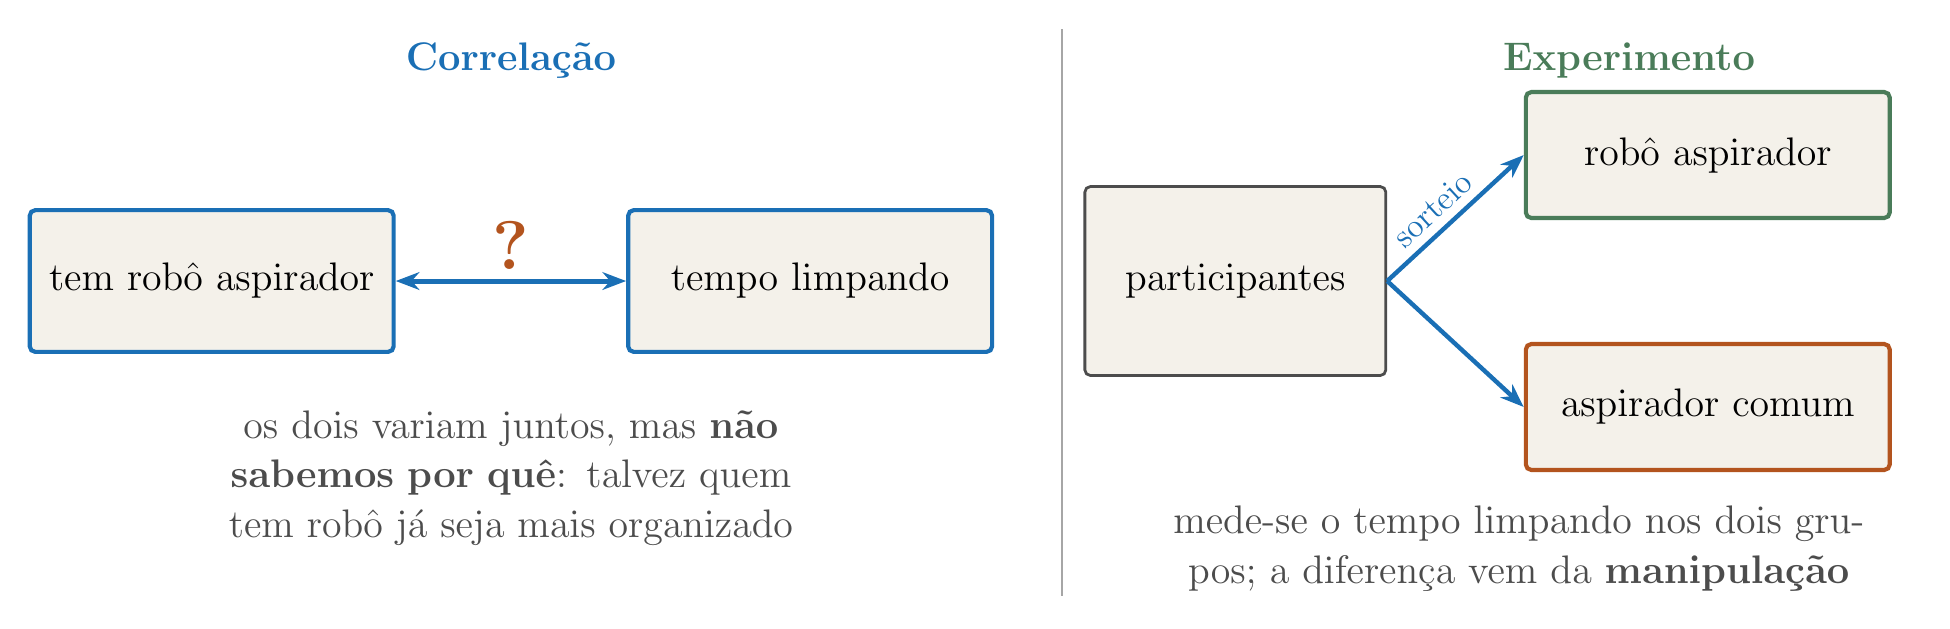
\begin{tikzpicture}[x=1cm,y=1cm]
  \node[font=\Large\bfseries, dblue] at (4.4,6.2) {Correlação};
  \node[dbox, text width=4.2cm, minimum height=1.8cm, font=\Large, draw=dblue, line width=1.5pt] (a) at (0.6,3.4) {tem robô aspirador};
  \node[dbox, text width=4.2cm, minimum height=1.8cm, font=\Large, draw=dblue, line width=1.5pt] (b) at (8.2,3.4) {tempo limpando};
  \draw[dtrans, line width=1.8pt, {Stealth[length=3mm]}-{Stealth[length=3mm]}] (a.east) -- (b.west) node[midway, above, font=\Huge\bfseries, dorange] {?};
  \node[font=\Large, black!70, align=center, text width=11cm] at (4.4,0.9) {os dois variam juntos, mas \textbf{não sabemos por quê}: talvez quem tem robô já seja mais organizado};
  \draw[black!35, line width=1pt] (11.4,-0.6) -- (11.4,6.6);
  \node[font=\Large\bfseries, dgreen] at (18.6,6.2) {Experimento};
  \node[dbox, text width=3.4cm, minimum height=2.4cm, font=\Large, draw=black!70, align=center] (s) at (13.6,3.4) {participantes};
  \node[dbox, text width=4.2cm, minimum height=1.6cm, font=\Large, draw=dgreen, line width=1.5pt, align=center] (g1) at (19.6,5.0) {robô aspirador};
  \node[dbox, text width=4.2cm, minimum height=1.6cm, font=\Large, draw=dorange, line width=1.5pt, align=center] (g2) at (19.6,1.8) {aspirador comum};
  \draw[dtrans, line width=1.6pt, -{Stealth[length=3mm]}] (s.east) -- (g1.west) node[midway, above, sloped, font=\large, xshift=-4pt] {sorteio};
  \draw[dtrans, line width=1.6pt, -{Stealth[length=3mm]}] (s.east) -- (g2.west);
  \node[font=\Large, black!70, align=center, text width=10cm] at (17.2,-0.0) {mede-se o tempo limpando nos dois grupos; a diferença vem da \textbf{manipulação}};
\end{tikzpicture}
\end{document}
